\newpage
\subsection{Goal}\label{subsec:goal}

The use of first- and second-order methods (Gradient Descent, Conjugate Gradient Descent, Newton's method and Levenberg-Marquardt algorithm) in the tasks of unconstrained nonlinear optimization.

\subsection{Formulation of the problem}\label{subsec:formulation-of-the-problem}

Generate random numbers $\alpha \in (0, 1)$ and $\beta \in (0, 1)$.
Furthermore, generate the noisy data $\{x_k, y_k\}$, where $k = 0, \dots, 100$, according to the following rule:

\begin{equation}
    y_k = \alpha x_k + \beta + \delta_k, x_k = \frac{k}{100},
\end{equation}

where $\delta_k \sim N(0, 1)$ are values of a random variable with standard normal distribution.
Approximate the data by the following linear and rational functions:

\begin{enumerate}
    \item $F(x, a, b) = ax + b$ (linear approximant),
    \item $F(x, a, b) = \frac{a}{1 + bx}$ (rational approximant),
\end{enumerate}

by means of least squares through the numerical minimization (with precision $\varepsilon = 0.001$ of the following function:

\begin{equation}
    D(a, b) = \sum^{100}_{k=0}(F(x_k, a, b) - y_k)^2.
\end{equation}

To solve the minimization problem, use the methods of Gradient Descent, Conjugate Gradient Descent, Newton's method and Levenberg-Marquardt algorithm.
If necessary, set the initial approximations and other parameters of the methods.
Visualize the data and the approximants obtained separately for each type of approximant.
Analyze the results obtained (in terms of number of iterations, precision, number of function evaluations, etc.) and compare them with those from Task 2 for the same dataset.

\subsection{Brief theoretical part}\label{subsec:brief-theoretical-part}

Optimization methods are numerical methods for finding optimal (in some sense) values of objective functions, for example, in the framework of mathematical models of certain processes.

\textit{First-and second-order optimization methods} use to minimize the objective function $f$ on the set $Q$ its value $f(x)$ and the values of its first and second derivatives (gradient, Hessian), respectively.

\paragraph{Gradient descent}

\textit{Gradient descent} is an optimization algorithm that's used when training a machine learning model.
It's based on a convex function and tweaks its parameters iteratively to minimize a given function to its local minimum.

\paragraph{Conjugate gradient method}

\textit{Conjugate gradient methods} represent a kind of steepest descent approach.
With steepest descent, minimization of a function begins $f$ starting at $x_0$ by traveling in the direction of the negative gradient - $f'(x_0)$.
In subsequent steps, the movement continues in the direction of the negative gradient evaluated at each successive point until convergence.

\paragraph{Newton's method}

\textit{Newton's method} is an iterative method for finding the roots of a differentiable function $f$, which are solutions to the equation $f(x) = 0$.
In optimization, Newton's method is applied to the derivative $f'$ of a twice-differentiable function $f$ to find the roots of the derivative (solutions to $f'(x) = 0$), also known as the stationary points of $f$.
These solutions may be minima, maxima, or saddle points.

\paragraph{Levenberg-Marquardt algorithm}

The \textit{Levenberg-Marquardt algorithm} (\textit{LMA}) is a popular trust region algorithm that is used to find a minimum of a function (either linear or nonlinear) over a space of parameters.
Essentially, a trusted region of the objective function is internally modeled with some function such as a quadratic.
When an adequate fit is found, the trust region is expanded.
As with many numerical techniques, the Levenberg-Marquardt method can be sensitive to the initial starting parameters.

\subsection{Results}\label{subsec:results}

It is known that optimization by \textit{linear approximation} has a unique solution, so these methods give similar optimal values for $a$ and $b$, regardless of the choice of initial approximations.
In the case of a \textit{rational approximation}, significant nonlinearities occur, so the result depends on the initial approximations (Figure~\ref{ris:plot}).

\begin{figure}[H]
    \center
    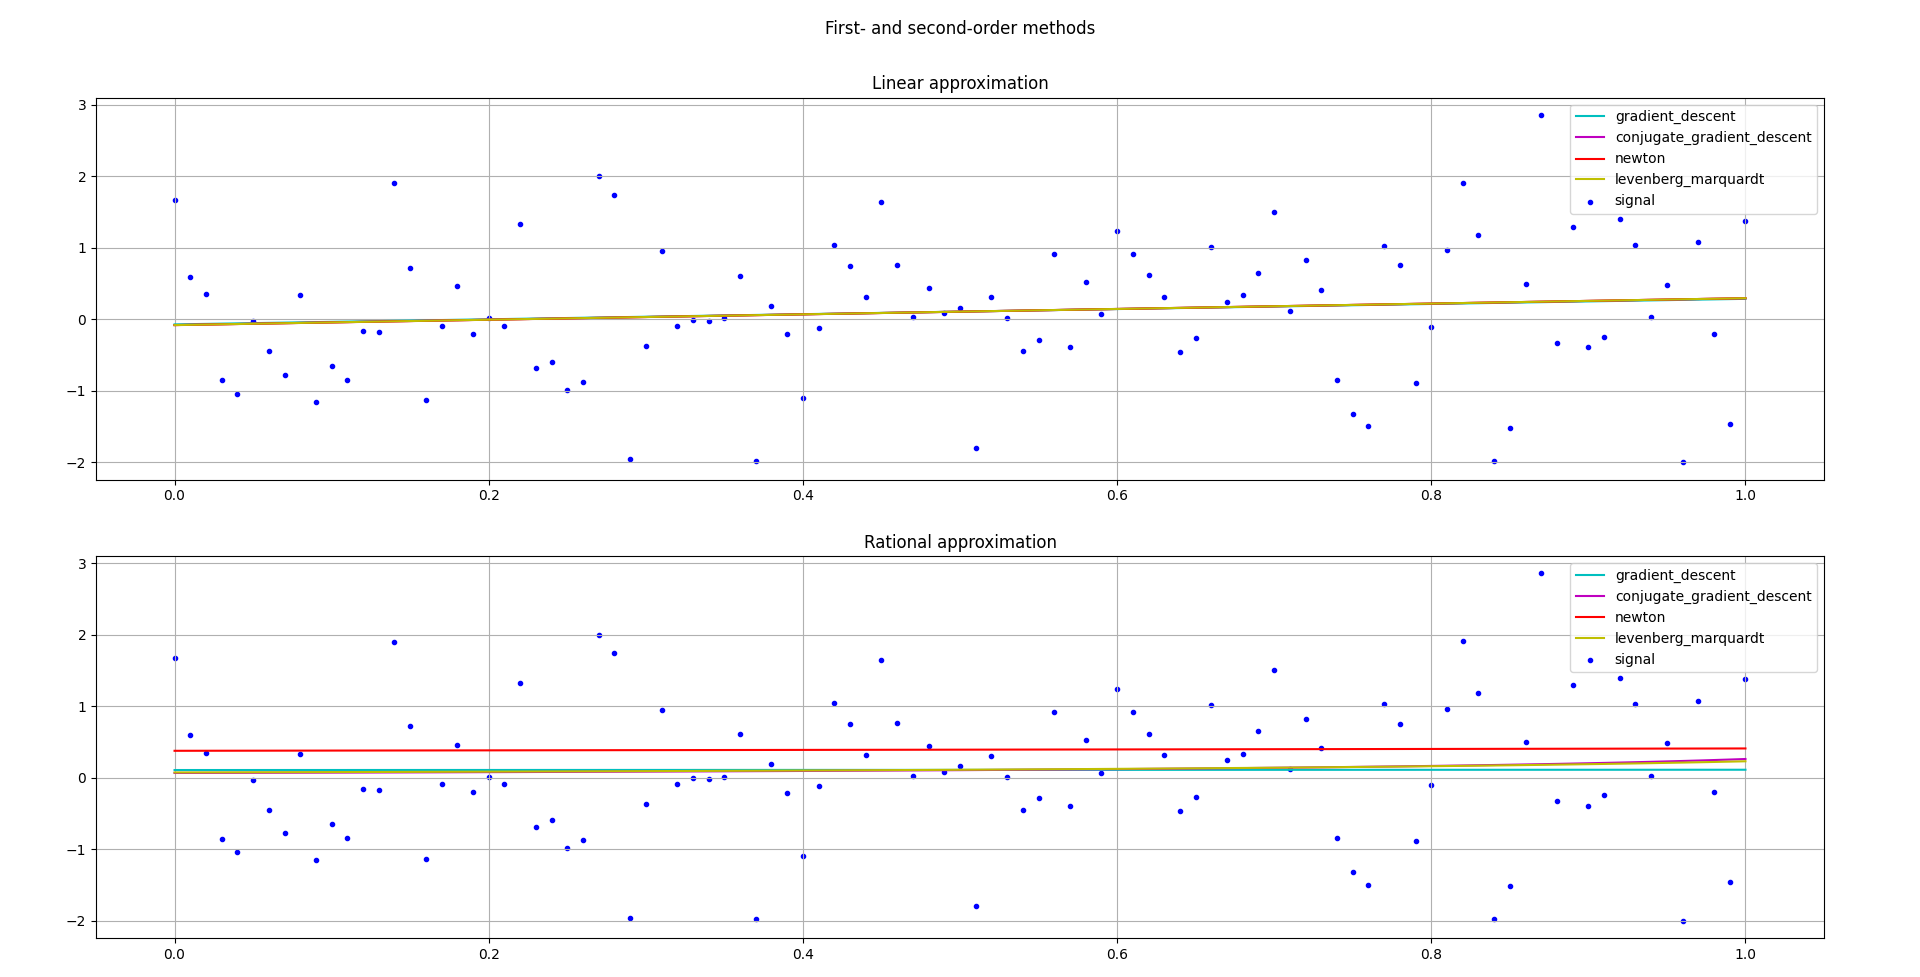
\includegraphics[width=\textwidth]{img/plot.png}
    \caption{Direct methods of optimization.}
    \label{ris:plot}
\end{figure}

From the tables below (Tables~\ref{tbl:direct},~\ref{tbl:order}), we can conclude that first-and second-order optimization methods require orders of magnitude less computational operations, in contrast to direct methods.

\begin{table}[ht]
\caption{Direct methods}
\begin{tabular}{l|l|l|l|}
\cline{2-4}
                                                & \textbf{method}             & \textbf{iterations} & \textbf{function eval} \\ \hline
\multicolumn{1}{|l|}{\multirow{3}{*}{\textbf{linear}}}   & exhaustive\_search & 5448000  & 5448000     \\ \cline{2-4}
\multicolumn{1}{|l|}{}                          & gauss\_method      & 77376     & 77376        \\ \cline{2-4}
\multicolumn{1}{|l|}{}                          & nelder\_mead       & 18         & 3             \\ \hline
\multicolumn{1}{|l|}{\multirow{3}{*}{\textbf{rational}}} & exhaustive\_search & 5448000  & 5448000     \\ \cline{2-4}
\multicolumn{1}{|l|}{}                          & gauss\_method      & 6448      & 6448         \\ \cline{2-4}
\multicolumn{1}{|l|}{}                          & nelder\_mead       & 10         & 2             \\ \hline
\end{tabular}
\label{tbl:direct}
\end{table}

\begin{table}[ht]
\caption{First- and second-order methods}
\begin{tabular}{l|l|l|l|}
\cline{2-4}
                                                         & \textbf{method}              & \textbf{iterations} & \textbf{function eval} \\ \hline
\multicolumn{1}{|l|}{\multirow{4}{*}{\textbf{linear}}}   & gradient\_descent            & 150                 & 150                    \\ \cline{2-4}
\multicolumn{1}{|l|}{}                                   & conjugate\_gradient\_descent & 80                  & 80                     \\ \cline{2-4}
\multicolumn{1}{|l|}{}                                   & newton                       & 250                 & 250                    \\ \cline{2-4}
\multicolumn{1}{|l|}{}                                   & levenberg\_marquardt         & 34                  & 34                     \\ \hline
\multicolumn{1}{|l|}{\multirow{4}{*}{\textbf{rational}}} & gradient\_descent            & 150                 & 150                    \\ \cline{2-4}
\multicolumn{1}{|l|}{}                                   & conjugate\_gradient\_descent & 104                 & 104                    \\ \cline{2-4}
\multicolumn{1}{|l|}{}                                   & newton                       & 208                 & 208                    \\ \cline{2-4}
\multicolumn{1}{|l|}{}                                   & levenberg\_marquardt         & 56                  & 56                     \\ \hline
\end{tabular}
\label{tbl:order}
\end{table}

\paragraph{Newton's method gives a different result}

\begin{theorem}
    \label{theorem:conv_newton}
    For doubly continuously differentiable functions (i.e.\ for $f \in C^2(D)$) with a non-degenerate matrix $\nabla^2 f(y^*)$, there exists a $\varepsilon$-neighborhood of the stationary point $y^*$ of the function $f(y)$ such that for any initial point $y^0$ from this neighborhood, the Newton method will converge superlinearly, and if the Lipschitz condition is met in this neighborhood for Hesse matrices, it will converge quadratically.
\end{theorem}

If we consider the Newton method in more detail, then we can conclude from the theorem above [1]: if the Hesse matrix is not degenerate, but not sign-positive, then the Newton method can converge to a stationary point that is not a minimum point, but a maximum point or a saddle point.
Accordingly, a more careful choice of initial approximations is necessary.

\subsection{Conclusion}\label{subsec:conclusion}

In the course of the laboratory work,  first- and second-order methods were implemented and analyzed within the problem of the unconstrained optimization problem.
This paper also provides a comparative analysis of direct optimization methods and first-and second-order methods.

\subsection{References}\label{subsec:references}
\begin{enumerate}[label={[\arabic*]}]
    \item С.Ю. Городецкий, Лабораторный практикум по методам локальной оптимизации в программной системе LocOpt, 2007.
\end{enumerate}

\subsection{Appendix}\label{subsec:appendix}

The source code is located \href{https://github.com/vanSultan/anal_dev_algo/tree/lab_03}{here}: \url{https://github.com/vanSultan/anal_dev_algo/tree/lab_03}.
